% =============================================================================
% CAPÍTULO 2 — volta 1 (AGENTS.md §6): o orçamento do alarme.
%
% O fracasso que o abre, com número na mão: o vigia do capítulo 1, ligado no limiar que
% o mundo parado nunca alcançou, soa sozinho uma vez a cada milhares de anos — e avisa
% do tombo de 2020 com 86% do prejuízo já pago.
%
% Medição: lab/experimentos/E02_orcamento.ipynb. Figuras: figuras/E02_orcamento_*.
% =============================================================================

\chapter{O orçamento do alarme}
\label{cap:orcamento}

\section{O vigia}

O capítulo anterior deixou um instrumento e um incômodo. O instrumento: contar quantas vezes
o preço rompeu a linha dentro de uma janela móvel de \numVigiaBloco{} dias. O incômodo: os
blocos têm data, e a média não vê a data.

A tentação, agora, é pequena e razoável. Se o bloco sabe \emph{quando} o mundo aperta, basta
transformá-lo num vigia: alarmar quando o bloco atingir um limiar. E o limiar já vem
escolhido por medição, não por gosto --- no capítulo anterior, o pior bloco de duzentos
mundos que nunca mudam chegou a \numNuncaMudaPiorBloco{} violações. Um número que o mundo
parado nunca alcançou é, no mínimo, um candidato honesto a linha de alarme.

Fica então o vigia mais simples que este livro consegue escrever: \emph{soa quando as
violações dos últimos \numVigiaBloco{} dias chegam a \numVigiaLimiar}.

Duas perguntas decidem se isso vale alguma coisa, e é delas que este capítulo trata: com que
frequência ele soa quando nada muda, e quanto tempo ele leva quando algo muda de verdade.

\section{Quanto ele soa quando nada muda}

A primeira pergunta só tem uma resposta honesta, e ela não vem do mercado: vem de mundos em
que nada muda. Sorteamos \numVigiaMundos{} séries do tamanho da nossa, com retornos
independentes e sempre com a mesma lei, submetemos cada uma ao mesmo corte, contamos os
blocos e perguntamos quantas vezes o vigia soaria.

No limiar \numVigiaLimiar{}, o resultado é \numVigiaDiasParadoPorMundo{} dia por mundo ---
praticamente nenhum ---, e \numVigiaMundosQueSoamPct\% dos mundos soaram pelo menos uma vez.
Em tempo: um alarme a cada \numVigiaAnosParadoPorAlarme{} anos de mundo parado.

É um número grande, e é preciso desconfiar dele. Ele se apoia em \numVigiaParadoAlarmes{}
alarmes em \numVigiaMundos{} mundos, e conta de evento raro não é precisa: o erro relativo é
de uns \numVigiaParadoErroPct\%. O que ela entrega é a ordem de grandeza --- milhares de
anos ---, não o número exato.

Há, porém, um jeito de conferir esse orçamento sem sortear nada, e vale escrevê-lo, porque
ele dá um teto \emph{provado}.

\begin{proposicao}[o teto independente]
\label{prop:teto}
Se os dias fossem independentes, com probabilidade $p$ de violar o corte em cada dia, então
a probabilidade de algum bloco de $B$ dias atingir $L$ violações não passaria de
$n \cdot \Prob\big(\text{Bin}(B, p) \geq L\big)$, onde $n$ é o número de blocos.
\end{proposicao}

\begin{proof}
O acontecimento \emph{algum bloco atinge o limiar} é a união, sobre os $n$ blocos, dos
acontecimentos \emph{este bloco atinge o limiar}. A probabilidade de uma união nunca excede a
soma das probabilidades dos seus termos, e sob independência a probabilidade de um bloco
atingir $L$ violações é a cauda da binomial.
\end{proof}

Com os números deste capítulo, o teto dá \numVigiaTetoIndependentePct\%. O mundo parado
mediu \numVigiaMundosQueSoamPct\%. O teto é honesto --- ele está acima --- e é frouxo por
quase uma dezena de vezes.

E há um limite para a utilidade dele: para limiares baixos a soma ultrapassa cem por cento e
o teto deixa de dizer qualquer coisa. Teto que vale cento e vinte por cento não é teto; é uma
conta que já não se aplica.

\section{Quanto ele demora quando algo muda}

O orçamento não diz nada sobre o que interessa. A pergunta que decide é outra: quando o mundo
muda de verdade, o vigia avisa a tempo de quê?

Aplicado à série inteira, no limiar \numVigiaLimiar{}, ele soou \numVigiaAlarmesReais{}
vezes: uma a cada \numVigiaAnosReaisPorAlarme{} anos. No mundo parado, o mesmo vigia soa uma
vez a cada \numVigiaAnosParadoPorAlarme{} anos. A razão entre os dois é de
\numVigiaRazaoRealContraParado{} vezes.

Isso responde a primeira metade da dúvida: neste limiar o vigia não é alarmista. A fração de
mundos parados que soam uma vez sequer num período deste tamanho é de
\numVigiaMundosQueSoamPct\%, de modo que se espera \emph{menos de um} alarme falso entre os
\numVigiaAlarmesReais{}. Quando ele soa, houve.

A segunda metade é a que dói. Para cada alarme, comparamos o dia em que ele soou com o topo
anterior e com o fundo seguinte --- o preço mais alto antes do tombo e o mais baixo depois
---, e medimos quanto do prejuízo \emph{já tinha acontecido} no dia do aviso.

Nos dois tombos maiores do período, o resultado é este.

\begin{table}[htbp]
  \centering
  \begin{tabular}{lrrr}
    \hline
    & atraso desde o topo & prejuízo já pago \\
    \hline
    alarme de \numVigiaTomboAntigoData & \numVigiaTomboAntigoAtrasoDias{} dias & \numVigiaTomboAntigoPagoPct\% \\
    alarme de \numVigiaTomboRecenteData & \numVigiaTomboRecenteAtrasoDias{} dias & \numVigiaTomboRecentePagoPct\% \\
    \hline
  \end{tabular}
  \caption{Os dois piores tombos do período, com o dia do alarme e a fração do prejuízo
    total que já tinha acontecido quando ele soou. No tombo mais recente, o alarme veio com
    \numVigiaTomboRecenteQuedaPct\% de queda já realizada, de um total de \numVigiaTomboRecenteTotalPct\%.}
  \label{tab:atraso}
\end{table}

A mediana dos \numVigiaAlarmesReais{} alarmes é de \numVigiaPagoMedianoPct\% de prejuízo já
pago. E em um deles o alarme soou exatamente no fundo, com \numVigiaPagoPiorPct\% do tombo
consumido: o vigia avisou no dia em que a queda acabou.

Vale dizer do modo mais direto possível. O vigia do capítulo anterior \emph{acerta}: os
alarmes dele são reais, e o mundo parado quase nunca o faz soar. O que ele não faz é
\emph{chegar antes}.

\section{A troca}

Se o vigia é tardio, a saída parece óbvia: baixar o limiar. Vale a pena medir, porque a saída
é ilusória e o preço dela tem forma.

Para cada limiar, medimos as duas coisas de uma vez: a frequência com que o vigia soa em
mundo parado, e o quanto do prejuízo já estava pago quando ele soou.

\begin{table}[htbp]
  \centering
  \begin{tabular}{rrr}
    \hline
    limiar & um alarme falso a cada & prejuízo já pago no tombo recente \\
    (violações) & (anos de mundo parado) & (\%) \\
    \hline
    \numTrocaOitoLimiar & \numTrocaOitoAnos & \numTrocaOitoPagoPct \\
    \numTrocaNoveLimiar & \numTrocaNoveAnos & \numTrocaNovePagoPct \\
    \numTrocaDezLimiar & \numTrocaDezAnos & \numTrocaDezPagoPct \\
    \numTrocaOnzeLimiar & \numTrocaOnzeAnos & \numTrocaOnzePagoPct \\
    \numTrocaDozeLimiar & \numTrocaDozeAnos & \numTrocaDozePagoPct \\
    \numVigiaLimiar & \numTrocaTrezeAnos & \numTrocaTrezePagoPct \\
    \hline
  \end{tabular}
  \caption{A troca, medida. Baixar o limiar antecipa o alarme e multiplica o falso alarme; a
    taxa de câmbio não é constante, e piora à direita da tabela.}
  \label{tab:troca}
\end{table}

A tabela diz três coisas.

\textbf{A troca existe, e o primeiro passo é barato.} Baixar o limiar de \numVigiaLimiar{}
para \numTrocaOitoLimiar{} derruba o prejuízo já pago de \numTrocaTrezePagoPct\% para \numTrocaOitoPagoPct\%: o
vigia passa a avisar antes de o tombo se completar. É a diferença entre saber e saber a
tempo.

\textbf{O preço desse passo é brutal.} O mesmo movimento leva o falso alarme de um a cada
\numTrocaTrezeAnos{} anos de mundo parado para um a cada \numTrocaOitoAnos{} anos. O vigia que
quase nunca se enganava passa a soar a cada poucos anos sem que nada tenha mudado.

\textbf{E a taxa de câmbio piora.} Na ponta direita da tabela, o limiar sobe de
\numTrocaDezLimiar{} para \numTrocaDozeLimiar, o falso alarme fica quase vinte vezes mais
raro, e o prejuízo já pago praticamente não se move: \numTrocaDezPagoPct\% contra \numTrocaDozePagoPct\%. Paga-se muito por nada. Há até
dois limiares vizinhos entregando exatamente a mesma coisa.

\begin{figure}[htbp]
  \centering
  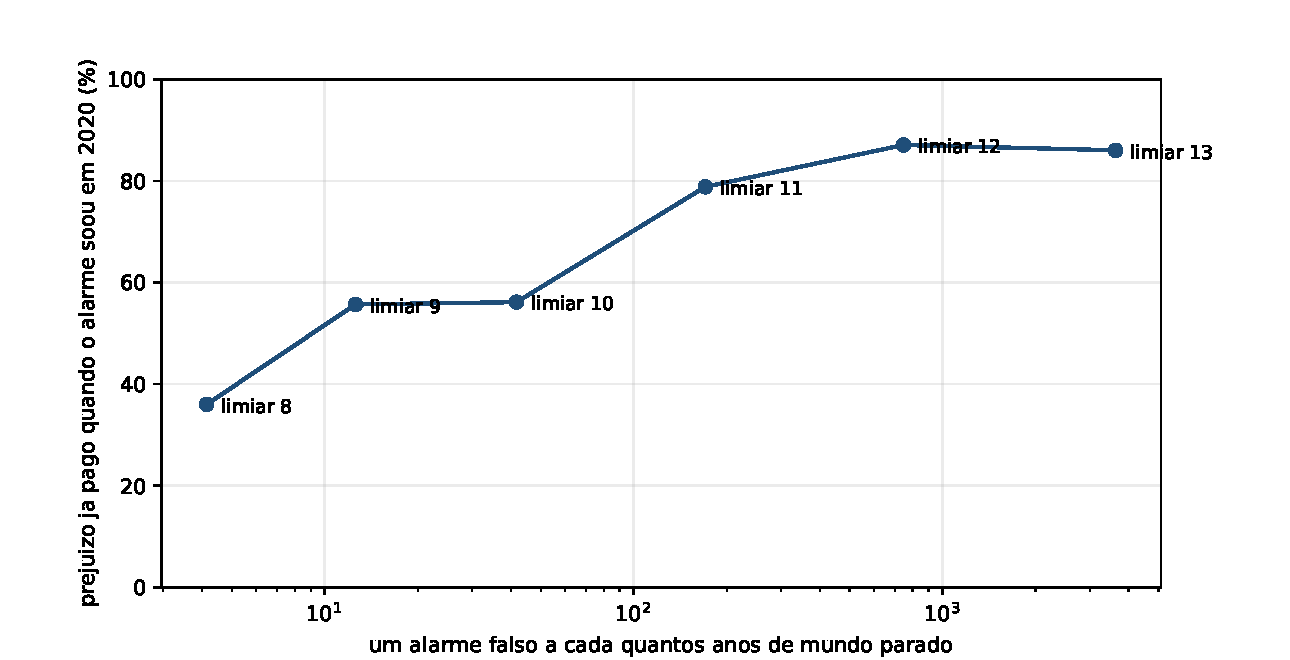
\includegraphics[width=\linewidth]{figuras/E02_orcamento_1.pdf}
  \caption{A troca em forma de curva: o eixo horizontal é a raridade do falso alarme, em
    escala logarítmica, e o vertical é o prejuízo já pago no tombo recente. A curva sobe depressa na
    esquerda e achata na direita.}
  \label{fig:troca}
\end{figure}

\emph{Não existe limiar que seja ao mesmo tempo raro e rápido.} O vigia é o par ---
frequência em mundo parado e atraso em mundo que muda ---, e escolher um limiar é escolher um
ponto dessa curva. Não há ponto que seja bom nos dois eixos.

\section{O piso}

Vale resistir à conclusão de que o vigia é mal calibrado, porque ele não é: ele está no chão
do que a sua própria aritmética permite.

\begin{proposicao}[o piso do atraso]
\label{prop:piso}
Um alarme que exige $L$ violações dentro da janela móvel não pode soar antes de $L$ pregões
depois de a mudança começar, se antes dela o corte não era violado.
\end{proposicao}

\begin{proof}
Para que a contagem chegue a $L$, são necessários ao menos $L$ dias com violação dentro da
janela. Cada dia com violação consome um pregão, e nenhum deles pode ser anterior ao começo
da mudança. Logo o alarme exige ao menos $L$ pregões.
\end{proof}

Com $L = \numVigiaLimiar$, o piso é de \numVigiaPisoPregoes{} pregões. E o alarme de
\numVigiaTomboRecenteData{} soou \numVigiaTomboRecenteAtrasoDias{} dias corridos depois do topo --- poucos pregões mais do que o
piso. O vigia não estava gastando tempo à toa; ele estava esperando a contagem encher, que é
o que ele sabe fazer.

A consequência é dura para quem queria melhorar o vigia ajustando números: a única alavanca
é o próprio limiar, e o limiar é o orçamento. Comprar velocidade é pagar em falso alarme, na
taxa de câmbio da \cref{tab:troca}.

\begin{figure}[htbp]
  \centering
  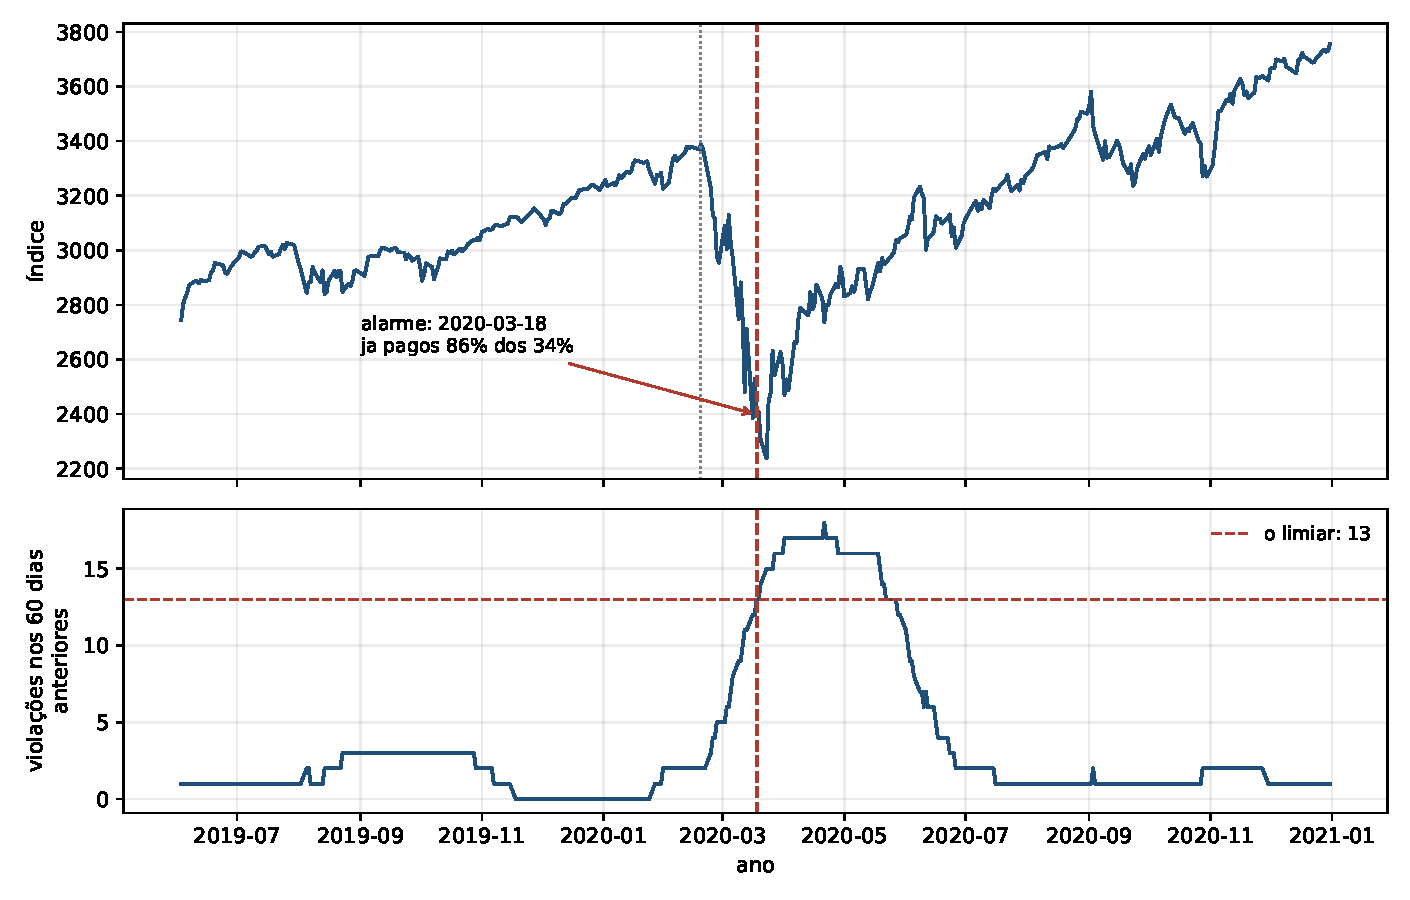
\includegraphics[width=\linewidth]{figuras/E02_orcamento_2.pdf}
  \caption{O alarme de \numVigiaTomboRecenteData{} visto dos dois lados. Em cima, o índice; embaixo, as violações
    dos \numVigiaBloco{} dias anteriores, com o limiar. As duas linhas contam a mesma
    história --- e a de baixo conta depois da de cima.}
  \label{fig:vigia2020}
\end{figure}

\section{O que fica}

Fica o orçamento, e ele é a peça que este capítulo veio buscar: \textbf{todo alarme é um par
declarado} --- com que frequência ele soa quando nada muda, e quanto ele demora quando algo
muda. Um alarme que não declara o par não é uma afirmação; é barulho com opinião. E o par não
se melhora por ajuste: a \cref{prop:piso} mostra que o atraso tem chão, e a
\cref{tab:troca} mostra quanto custa descer.

É este o orçamento que as quatro famílias de perguntas deste livro vão usar: em cobertura,
em proteção, em capacidade e em memória, a mesma pergunta aparece --- o que se promete, o que
se entrega, e quanto custa a diferença.

E fica o fracasso seguinte, que é o mais fundo até aqui. Este vigia conta \emph{uma forma} de
mudança: a que engorda a contagem de violações. Uma mudança que nunca rompe a linha é
invisível para ele em \emph{qualquer} limiar. Se o que mudou foi o tamanho da cauda --- dias
um pouco piores, sem que nenhum rompa o corte ---, se foi a dependência entre duas séries que
antes andavam separadas, ou se foi o calendário, com as coisas ruins passando a se juntar na
mesma semana, a contagem não se mexe e o vigia não soa.

A pergunta que fica, então, não é como calibrar melhor este vigia: é \emph{que formas a
mudança tem}, e como se mede cada uma delas com um orçamento comparável. É para lá que o
livro vai agora.
